\chapter{扩展}
这个章节解释开发者如何增加功能到TensorFlow。
\section{TensorFlow架构}
我们设计TensorFlow是为了大规模分布式训练和推理,但是它也能灵活的支持一些新的机器学习模型实验和系统级别的优化。

这个文件描述了这个系统架构使得结合这个规模和灵活度成为可能。假设你熟悉TensorFlow基本的一些概念,像计算图,操作绘画。
这个文档适合于那些想用当前API不支持的一些方法扩展TensorFlow,想要优化TensorFlow的硬件工程师,在法规莫分布式系统上实现机器学习系统或者是任何想要了解TensorFlow的hood的人。读完它后你应该能读和修改TensorFlow核心代码。
\section{概述}
TensorFlow运行时是一个跨平台的库,下图画出了常用的架构,C API分隔用户代码和核心代码。
\begin{center}
\begin{figure}[H]
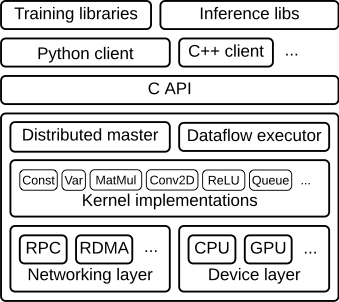
\includegraphics{layers.png}
\end{figure}
\end{center}
\begin{itemize}
\item \textbf{Client}
\item 定义计算作为数据流图。
\item 用session初始化图。
\item Distributed Master
\item 从图中修剪一个子图作为定义的参数给Session.run()
\item 分开不同的子图为多个部分在不同的进程和设备上运行。
\item 分配图块到worker service。
\item \textbf{Worker services}
\item 调度图上的操作在可用的硬件平台(CPUs,GPUs)上执行。
\item 发送和接收worker service的操作结果。
\item 内核实现。
\item 执行单个图操作的计算。
\end{itemize}
下图说明逐渐的交互。"job:worker/task:0"和"/job:ps/task:0"两个任务在wokers上。"PS"代表"parameter server":一个负责存储更新模型参数的任务。另一个任务优化参数时发送更新到这些参数,类似的在任务之间的分隔是不被要求的,但是它通常用于分配的训练。
%没有图像
\begin{figure}[H]
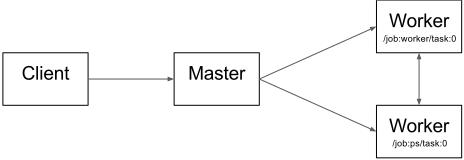
\includegraphics{diag1.png}
\end{figure}
注意Distributed Master和Worker Service仅仅存在于分布的TensorFlow。,单进程版本的TensorFlow包含一个特别的Session实现能做任何Distributed msdter能做的不仅仅是和本地进程通信。

下面的章节表述了TensorFlowlayer的核心。
\subsection{Client}
用户写TensorFlow程序构造计算图。这个车给需既可以直接组成单个操作或者用一个像Estimators API的方便的库组成神经网络乘和其他高级抽象。TensorFlow支持多种用户语言,但是我们优先使用Python和C++,仅仅是因为我们的内部用户熟悉他们。当特征被建立好后我们将他们接入C++。因此用户可以得到一个对所有语言优化的实现。大多数的训练库仅仅支持Python,但是C++支持更高效的推理。
用户创建一个绘画,发送图的定义到ditributed master作为tf.GraphDef 协议缓冲区。然后客户评估图上的一个节点或者多个节点,评估触发一个distributed master的调用初始化计算。

在下图中,客户建立一个图,应用权重(w)到特征向量(x),增加偏置(b)保存结果。
%没有图像
\begin{figure}[h]
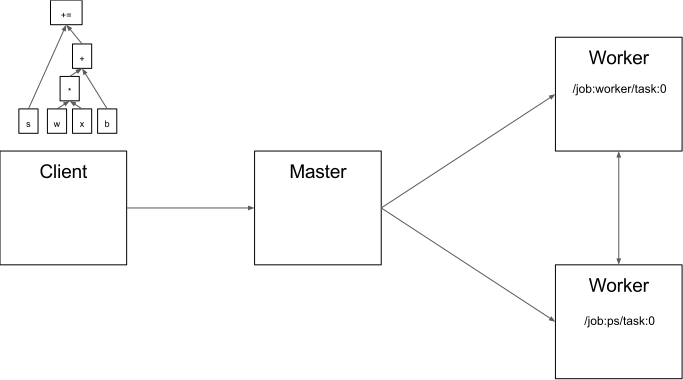
\includegraphics[scale=0.5]{graph_client.png}
\end{figure}
\subsection{Distributed master}
\begin{itemize}
\item 修剪图得到子图计算用户的节点请求。
\item 对于每一个加入的设备,分隔图获得子图。
\item 缓存这些块以至于他们能用在自序列中。
\end{itemize}
因为master查看每一步的计算,它用像常用的子表达式消除和常数折叠的标准的优化。它然后执行优化的子图。
下图显示一个可能的分隔。distributed master有组合的模型参数为了放置他们在参数服务器上。
这里图的边缘被分隔,distributed master发送接收节点在不同的任务间传送信息。
下面的distributed master传输子图到分布的任务。
\subsection{Worker Service}
任务中的worker service。
\begin{itemize}
\item 处理master的请求。
\item 调度内核执行包含本地子图的操作
\item 任务间的直接通信。
\end{itemize}
我们偶化worker service为了能用更小的花销以女性大的图。我们当前的实现能实现每秒执行上万张子图,使得大量的副本快速的训练。worker service布置内核到本地设备上然后通过利用多CPU多GPU尽可能的并行执行。
我们为源和目的设备指定发送和接收操作。
\begin{itemize}
\item 用cudaMemcpyAsync() API在本地CPU和GPU之间转换,覆盖计算和数据的转化。
\item 用对等的DMA在不同的本地GPU之间转化避免通过主CPU的高昂代价。
\end{itemize}
对于任务间的转化,TensorFLow用多个协议,报错:
\begin{itemize}
\item gPRC over TCP
\item RDMA over COnverged Ethernet
\end{itemize}
我们对于NVIDIA的多GPU通信NCCL库有初步的支持,查看\href{}{tf.contrib.nccl}
\section{内核实现}
运行包含超过200个标准操作白扩数学,数组操作,控制流,状态管理操作。每一个操作对不同的设备有优化,一些操作内核用Eigen::Tensor实现,用C++模板生成在多核CPU和GPUs上生成高效的并行代码,然而我们优先像像CuDNN这类更高效实现的库。我们也实现了量化,能在移动设备和高流通数据中心应用上更快地推理,用gemmlowp地精读矩阵库加速量化计算。

如果很难或者抵消的表达子计算作为操作的组成,用户可以注册额外的京城通过C++提供更高效的实现,,我们推荐你duit一些重要的操作像ReLU和Sigmoid和相关的梯度注册你的融合内核,XLA变压器有意额实验性是实现自动内核融合。

